\documentclass{article}

\usepackage{enumerate}
\usepackage{kbordermatrix}
\usepackage{graphicx}
\usepackage[font=small,labelfont=bf]{caption}
\usepackage{amsmath}
\usepackage{amsfonts}
\usepackage{amssymb}
\usepackage{amsthm}
\usepackage{algorithm2e}
\usepackage{tikz}
\usetikzlibrary{automata, positioning, arrows, calc}

\title{Frequentist and Bayesian Analyses of the Board Game \textit{Outlaw}}
\author{Jediah Katz}
\date{February 21, 2018}

\renewcommand{\qed}{$\hfill \blacksquare$}
\newcommand{\T}{\textbf{\textit{T}}}
\newcommand{\x}{\vec{x}}
\renewcommand{\arraystretch}{1.3}

\theoremstyle{definition}
\newtheorem{defn}{Definition}
\theoremstyle{plain}
\newtheorem{thm}{Theorem}

\begin{document}
	\maketitle
	\pagenumbering{arabic}
	\begin{abstract}
		A variant of the dice-based board game \textit{Outlaw}, designed by Phil Horswell, was analyzed 
	\end{abstract}

	\section{Background}
	Two of the most prominent understandings of probability are the frequentist and Bayesian interpretations. Frequentist probability, most generally, defines probability as the relative frequency of an event's occurrence in a suitable number of repetitions of a process. In contrast, Bayesian probability, most generally, defines probability as the degree of confidence in an event's occurrence held by a suitable agent. Each of these interpretations of probability corresponds to its own means of modeling a process in order to determine the probability that particular events will occur.
	
	\subsection{Monte-Carlo Simulations}
	Imagine a rather boring game in which a single player rolls one die each turn and adds its value to the the score, which begins at zero. The player wins if the score is greater than twenty after five turns, and loses otherwise. Suppose we are interested in determining the probability that the player wins the game. In the frequentist interpretation of probability, an intuitive solution is to simply play the game many times, recording whether the player wins or loses.
	
	However, it is often impractical and time-consuming to manually repeat this process a suitable number of times in order for the relative frequency to converge. Fortunately, the use of a computer can greatly speed up the repetition of trials. By creating a simulation to model the playing of a game, millions of trials can be run in very little time, a process known as the Monte-Carlo method. 
	
	It is worth noting that assumptions must often be made in the process of building a computer simulation. For example, in order to simulate the rolling of a die, we assume that a uniform pseudo-random number generator that generates integers in the interval {[1,6]} correctly models the behavior of a die.
	
	\subsection{Absorbing Markov Chains}
	For some more complex processes, however, even a computer simulation may not be feasible. Events with very low probability, such as ten dice each rolling a six, can easily require hundreds of millions of trials to occur in a simulation. Fortunately, Bayesian methods of probability modeling provide an elegant solution to this problem. As Bayesian probability is not constrained by the idea of frequency, we can use our assumptions to mathematically model processes.


	One of the most valuable tools for modeling in the Bayesian's belt is the Markov chain. 

\begin{defn}
For some finite state space $I$, we define a discrete-time Markov chain with initial distribution $\lambda$ and transition matrix $\T$ as a  sequence of random variables $(X_n)_{n \geq 0}$ such that, for $n \geq 0$ and $i_0, \dots, i_{n+1} \in I$,
	\begin{enumerate}[(i)]
	\item $\lambda_{i_0} = \Pr[X_0 = i_0]$  
	\item $\T_{i_n, i_{n+1}} = \Pr[X_{n+1} = i_{n+1} ~|~ {X_0 = i_0}, \dots, X_{n}=i_n]$

	\hspace{3.7em}$ = \Pr[X_{n+1} = i_{n+1} ~|~ X_{n} = i_n]$
	\end{enumerate}
\end{defn}
We can represent $(X_n)_{n \geq 0}$ with the convenient notation $Markov(\lambda, \T)$. Equivalent to (ii), the probability of transitioning to state $j$ from state $i$ is given by $\T_{i, j}$ and is independent of all previous states; this is known as memorylessness or the Markov property. Also, note that $\T$ is a right stochastic matrix, meaning that for any $i \in I$, \[\sum_{j\in I} \T_{i, j} = 1;\] that is, the probabilities in each row of $\T$ sum to 1. Finally, note that we represent the distribution $\lambda$ as a stochastic vector.
\\
	
	An absorbing Markov chain is simply a Markov chain for which there exists a state $i \in I$ such that $\T_{i,i} = 1$. Equivalently, an absorbing Markov chain contains at least one state from which transition to another state is impossible. Absorbing Markov chains are especially useful for modeling games, as winning a game is typically an absorbing state.
	
	Consider the game represented by the directed graph below. The player begins at state $a$. Each turn, the player rolls a die and then transitions across the corresponding edge, if one exists. The player wins upon reaching state $c$.
	
	\[
	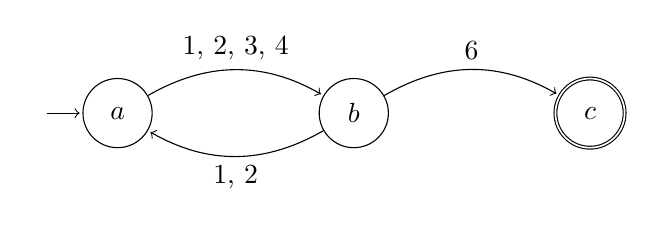
\begin{tikzpicture}[shorten >=1pt, node distance=3cm,auto, initial text={}]
      \node[state,initial] (a) {$a$};
      \node[state] (b) [right of=a] {$b$};
      \node[state,accepting] (c) [right of=b] {$c$};
      \path[->]
                (a) edge[bend left] node {1, 2, 3, 4} (b)
                (b) edge[bend left] node {6} (c)
                (b) edge[bend left] node {1, 2} (a);
     \end{tikzpicture}
	\]
	
	Since the probability of transitioning between states only depends on the current state, this game is an ideal candidate for a Markov chain with state space $I = \{a, b, c\}$. Since the player begins at state $a$ with probability 1, then we can represent this game as a Markov-chain $Markov(\lambda, \T)$ such that
	\[\lambda = \kbordermatrix{ ~ &a &b &c \cr
		& 1 & 0 & 0},\]
	\[\T = \kbordermatrix{~ &a & b & c \cr
		a&\frac{2}{6} &  \frac{4}{6}  & 0 \cr
		b& \frac{2}{6}  &  \frac{3}{6} & \frac{1}{6} \cr
		c& 0 & 0 & 1}\]
	At this point, it is very simple to determine the probability that the player is at any state in $i \in I$ after $n$ turns, for some $n \in \mathbb{N}$.
\\
	\begin{thm}
	If $(X_n)_{n \geq 0}$ is $Markov(\lambda, \T)$, then for all $n \geq 0$, $i_0, \dots, i_n \in I$, \[\Pr[X_0 = i_0, X_1 = i_1, \dots, X_n = i_n] = \lambda_{i_0}\T_{i_0, i_1}\T_{i_1,i_2}, \dots, \T_{i_{n-1}, i_n}\]
	\end{thm}
	
	\begin{proof} Since $(X_n)_{n \geq 0}$ is $Markov(\lambda, \T)$, then
	\begin{align*}
	\Pr[&X_0 = i_0, X_1 = i_1, \dots, X_n = i_n]\\
	 &= \Pr[X_0 = i_0]\Pr[X_1 = i_1 | X_0 = i_0]\dots\Pr[X_n = i_n | X_0 = i_0, \dots X_{n-1} = i_{n-1}]\\
	 &= \lambda_{i_0}\T_{i_0, i_1}\T_{i_1,i_2}, \dots, \T_{i_{n-1}, i_n}
	\end{align*}
	\end{proof}
	It can be shown that the converse of this statement holds as well.
	
	\begin{thm} If $(X_n)_{n \geq 0}$ is $Markov(\lambda, \T)$, then for any $n \geq 0$, $j \in I$,
	\[\Pr[X_n = j] = (\lambda \T^{\,n})_j\]
	\end{thm}
	
	\begin{proof}
	The probability $\Pr[X_n = j]$ that we are on state $j$ after $n$ steps is equal to the sum of the probabilities of each permutation of states from steps $0$ through $n-1$. Therefore,
	\begin{align*}
	\Pr[X_n = j] &= \sum_{i_0 \in I} \dots \sum_{i_{n-1} \in I} \Pr[X_0 = i_0, \dots, X_{n-1} = i_{n-1}, X_n = j]\\
	&= \sum_{i_0 \in I} \dots \sum_{i_{n-1} \in I} \lambda_{i_0}\T_{i_0, i_1}\dots\T_{i_{n-1}, j} \tag{by Theorem 1}\\
	&= (\lambda \T^n)_j
	\end{align*}
	\end{proof}
	
		Returning to our game, we can use this identity to determine the probability of being at each state after ten turns.
		\begin{align*}
		\Big[\Pr[X_{10} = i] ~|~ i \in I\Big] &= 
		\begin{bmatrix}
		\Pr[X_{10} = a] & \Pr[X_{10} = b] & \Pr[X_{10} = c]
		\end{bmatrix}\\ &=
		\begin{bmatrix}
		1 & 0 & 0
		\end{bmatrix}
		\begin{bmatrix}
			\frac{2}{6} & \frac{4}{6} & 0           \\
			\frac{2}{6} & \frac{3}{6} & \frac{1}{6} \\
			0           & 0			  & 1
		\end{bmatrix}
		^{10}\\
		&=	
		\begin{bmatrix}
		\frac{1033729}{7558272} & \frac{3486025}{15116544} & \frac{3187687}{5038848}
		\end{bmatrix}
		\approx \begin{bmatrix}
		.14 & .23 & .63
		\end{bmatrix}
		\end{align*}
	\\
	Thus $\Pr[X_{10} = a] \approx .14$, $\Pr[X_{10} = b] \approx .23$, and $\Pr[X_{10} = c] \approx .63$.
	
	\subsection{The \textit{Outlaw} Game}
	We analyze a variant of \textit{Outlaw}, a dice-based board game intended for 2 to 3 players, designed and published online by Phil Horswell. The \textit{Outlaw} game board features the set of 12 outlaws $O = \{o_4, \dots, o_{9}, o_{19}, \dots, o_{24}\}$, each with a unique identifier in the range $[4, 9] \cup [19, 24]$. Players take turns rolling 4 dice; if the sum of the dice is equal to $k$ for $k \in [4, 9] \cup [19, 24]$, then the player captures outlaw $o_k$. Each outlaw comes with an associated cash bounty.
	
	\begin{center}
	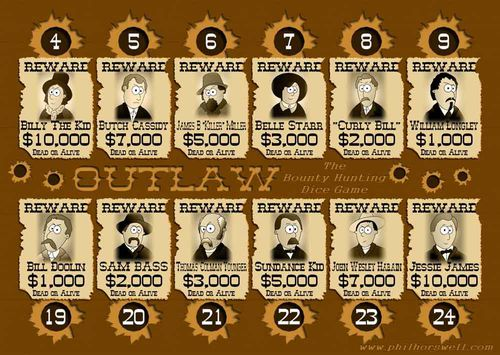
\includegraphics[scale=0.5]{outlaw_board}
	\captionof{figure}{The \textit{Outlaw} game board.}
	\end{center}
	
	In our ``Jailbreak'' variant of the game, if a player $P$ rolls an outlaw who has already been captured by a distinct player $P'$, then $P$ will steal that outlaw from away from $P'$. Only one player can have possession of any particular outlaw at one time. If a player $P$ has possession of $n$ distinct outlaws at once, then $P$ wins the game.
	
	\begin{defn}
	We let $G = Jailbreak(p, n)$ be  a game of ``Jailbreak'' \textit{Outlaw} such that $G$ has $p$ players, and a player $P$ wins if $P$ has possession of $w$ distinct outlaws at once.
	\end{defn}
	
	\section{Analysis of $Jailbreak(p, w)$}

	We begin by analyzing $G = Jailbreak(p, w)$. Our analysis centers upon the length of the game; that is, how many turns are required in expectation until any player wins?

	\subsection{Frequentist Analysis}
	We present the following psuedocode to simulate a run of $G$. The actual code is available in the resources folder; C++ was used for its speed. Note that we define a maximum number of turns to ensure that the procedure terminates.
	\begin{algorithm}
	\SetKwInOut{Input}{Input}
	\Input{$p$ : number of players\\ $w$ : number of outlaws to win\\ $m$ : maximum number of turns}

	\SetKwInOut{Output}{Output}
	\Output{number of turns in simulated run of $Jailbreak(p, w)$}
	\ForEach{outlaw $o$}{
		owner[$o$] $\gets$ None
	}
	\ForEach{player $P$}{
		numOutlaws[$P$] $\gets$ 0
	}
	turn $\gets$ 0\\
	\While{turn $< m$}{
		turn $\gets$ turn + 1\\
		\ForEach{player $P$}{
			$k \gets$ randInt(1, 6) + randInt(1, 6) + randInt(1, 6) + randInt(1, 6)\\
			\If{$4 \leq k \leq 9$ or $19 \leq k \leq 24$}{
				numOutlaws[$P$] $\gets$ numOutlaws[$P$] + 1\\
				prevOwner $\gets$ owner[$o_k$]\\
				\If{{\upshape oldOwner} not \upshape None}{
					numOutlaws[prevOwner] $\gets$ numOutlaws[prevOwner] - 1
				}
				owner[$o_k$] $\gets P$\\
				\If{{\upshape numOutlaws[$P$]} $\geq w$}{
					\Return{\upshape turn}
				}
			}
		}
	}
	\Return{``turn limit reached''}
	\end{algorithm}

	\subsection{Bayesian Analysis}
	% Todo: explain why we only keep track of player 1's state
We attempt to construct a Markov chain $(X_n)_{n \geq 0} = Markov(\lambda, \T)$ to describe $G$. We must first choose an appropriate state space $I$. Clearly, we cannot let a state simply represent the number of outlaws that $P_1$ controls, because different outlaws have different probabilities of capture, so it matters precisely which outlaws $P_1$ controls.  Therefore, we let $I = \{S \in \mathcal{P}(O) ~\big|~ |S| \leq w\}$; that is, each state represents the subset of distinct outlaws that $P_1$ controls. We don't need to consider subsets of more than $w$ outlaws, because once $P_1$ collects $w$ outlaws then the game is over.

	% Future note - we can simplify all of the n-subsets into one state!
	Now that we have chosen our state space, we must choose our initial distribution $\lambda$. At the start of the game, each player controls no outlaws; therefore, \[\lambda_\emptyset = \Pr[X_0 = \emptyset] = 1, \text{ and }\lambda_S = \Pr[X_0 = S] = 0,\] for all $S \in I$ s.t. $S \neq \emptyset$.
	
	\begin{thebibliography}{9}
		\bibitem{interpretations}
		H\'{a}jek, Alan, ``Interpretations of Probability'', The Stanford Encyclopedia of Philosophy (Winter 2012 Edition), Edward N. Zalta (ed.), \texttt{https://plato.stanford.edu/archives/win2012/entries/probability-interpret/}.
	\end{thebibliography}
\end{document}